\hypertarget{jour-j-faire-le-pont-entre-loccident-et-lorient}{%
\section{Jour J : faire le pont entre l'Occident et
l'Orient}\label{jour-j-faire-le-pont-entre-loccident-et-lorient}}

Ca y est ! Après les derniers préparatifs (sportifs), nous avons laissé
derrière nous notre chez-nous. Le Liban nous attend pour le début de ce
périple.

\begin{figure}
\centering
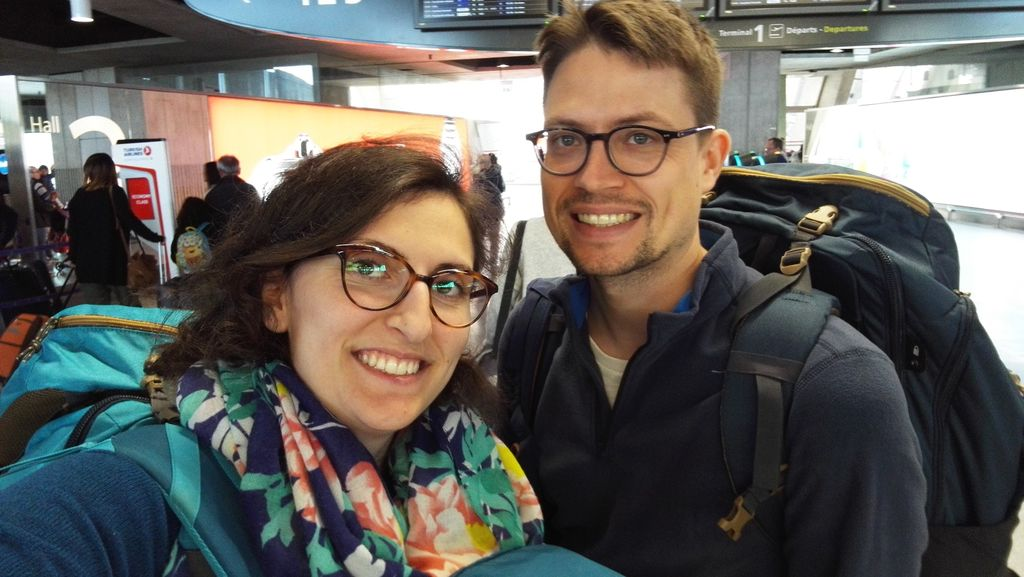
\includegraphics{images/20180503_depart.jpg}
\caption{Selfie-sac à dos de rigueur.}
\end{figure}

Est-ce qu'on réalise ce qui nous arrive ? Pas vraiment. Est-ce qu'on est
stressés ? Un peu. Une chose est sûre : on est contents :D

\begin{figure}
\centering
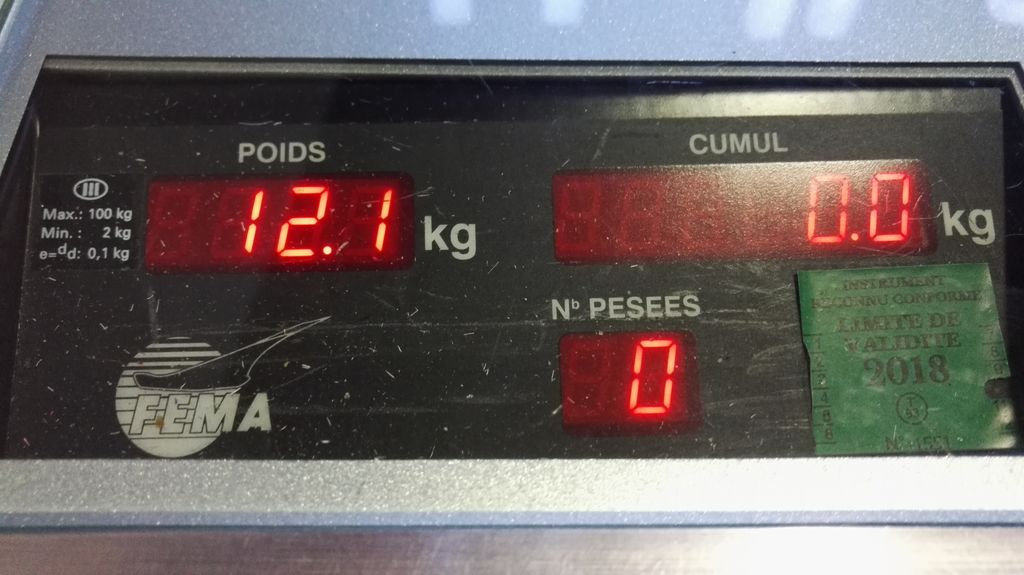
\includegraphics{images/20180503_Elida_sac.jpg}
\caption{Pour ceux qui n'y croyaient pas : elle l'a fait (ou presque...
aïe les 100 grammes de trop !).}
\end{figure}

\begin{figure}
\centering
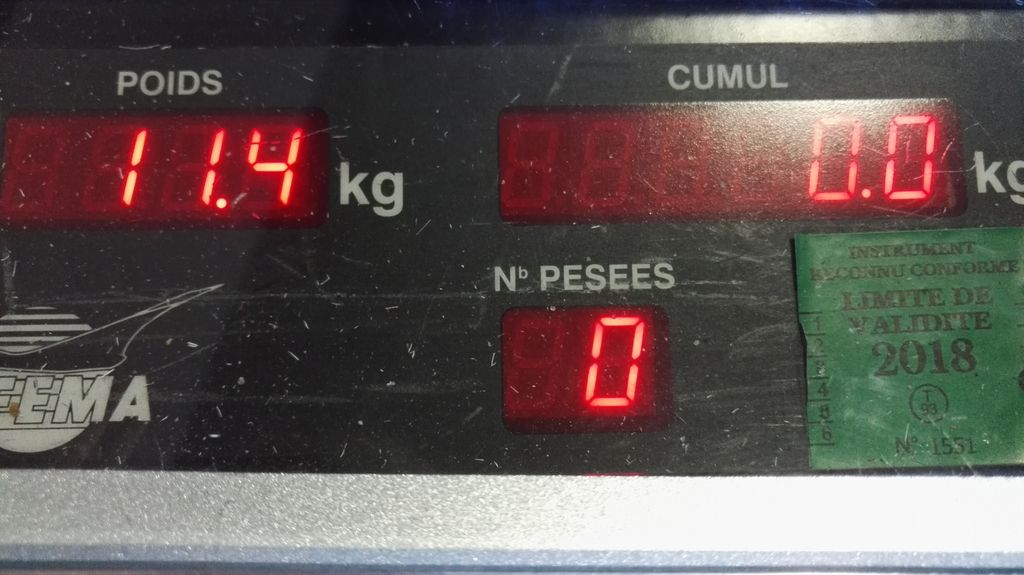
\includegraphics{images/20180503_Florian_sac.jpg}
\caption{Florian 1 - Elida 0.}
\end{figure}

Et devinez d'où on écrit ce billet ? Istanbul, première escale d'une
longue série. On fait pas mieux comme transition entre les continents !

\begin{figure}
\centering
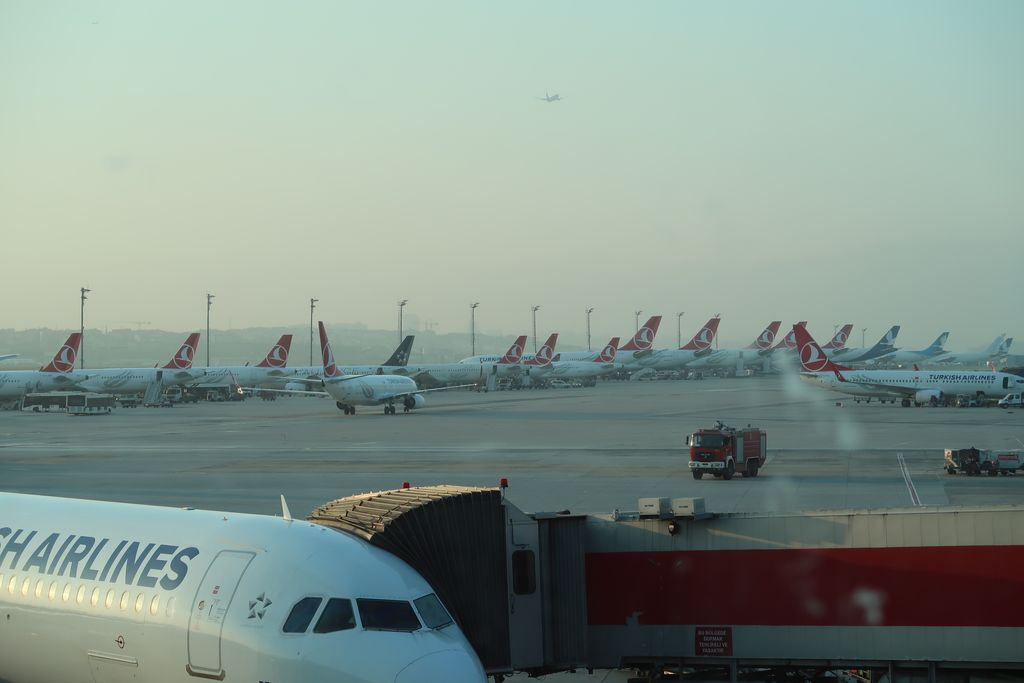
\includegraphics{images/20180503_Escale_Istanbul.JPG}
\caption{Le soleil se couche maintenant sur l'aéroport d'Istanbul (et
Flo ne rate pas une occasion de s'entraîner avec l'appareil photo ;) ).}
\end{figure}

Vite, on embarque. A très vite !

\emph{Elida et Florian}
